\chapter{Introdução}
\label{cap:introducao}


\begin{flushright}
``Ordinary life is pretty complex stuff.''\\
(Harvey Pekar)
\end{flushright}

Os sistemas complexos compreendem um campo interdisciplinar da ciência que não possui uma definição exata. Este conjunto amplo de fenômenos é comumente identificado e agrupado por algumas de suas características: são formados pela contribuição de um conjunto (geralmente grande) de componentes (muitas vezes simples) que, interagindo, estruturam-se de forma auto-organizada, gerando resultados inesperados, que não podem ser previstos pelos estudos estatísticos e/ou matemáticos tradicionais dos elementos formadores do sistema.

Na área dos estudos ambientais, os sistemas complexos possuem diversas aplicações: sistemas de transportes, redes de energia e comunicação, organizações sociais e econômicas, densidade e ocupação humana do espaço, dentre outas. Os estudos do clima e de variáveis meteorológicas ocupam um espaço de particular relevância na intercessão entre os estudos ambientais e os sistemas complexos. Em 2021, a Academia Real das Ciências da Suécia concedeu metade do Prêmio Nobel de Física para Syukuro Manabe e Klaus Hasselmann, cujos estudos apresentam modelos complexos para a análise do clima. Em particular apontam uma correlação entre as emissões de dióxido de carbono e as mudanças climáticas.

Muitos fenômenos complexos são investigados pela análise de grandes conjuntos de dados. É notável a velocidade e quantidade de dados que são gerados e armazenados pela humanidade atualmente. A aquisição, manipulação, gestão, armazenamento e criação de valor a partir de dados, através de ambientes computacionais, tem-se apresentado como um novo paradigma tecnológico. Um campo do conhecimento que recebeu a denominação de Ciência de Dados, conceito que envelopa alguns termos frequentemente associados à inovação científica, técnica e social como \emph{Big Data}, mineração de dados, \emph{Business Intelligence} internet das coisas, inteligência artificial e aprendizado de máquina(AM), dentre outros \cite[p. 12-13]{EMCdata2015}.

Uma das formas em que os dados costumam ser organizados são as denominadas séries temporais. As séries temporais são definidas como um conjunto de observações (numéricas ou categóricas) ordenado no tempo.  Embora muitos dos dados que descrevem as dinâmicas espaciais podem ser registrados na forma de sérias temporais (abastecimento de água nas tubulações, consumo de energia elétrica nos imóveis, fluxos de pessoas e veículos pela cidade, casos de uma doença por dia, etc.), contudo as técnicas de medição de correlações, bem como a devida exploração destas para inferir novos conhecimentos, permanecem como perguntas abertas em muitas sub-áreas das ciências ambientais\cite{Bermudez-Edo2018}.

Esta pesquisa propõe-se um estudo de dois conjuntos de variáveis meteorológicas, utilizando o \dmc como ferramenta de medição das correlações entre múltiplas variáveis. Após a avaliação dos resultados destes estudos, propõe-se a criação de um modelo preditivo utilizando ferramentas de AM e o \dmc.

\section{Definição do problema}
\label{sec:problema}

Os fenômenos climáticos apresentam as características dos sistemas complexos. Um sistema integrado, envolvendo aspectos globais e as condicionantes planetárias, fatores locais de cobertura da terra, proximidade de corpos d'agua, regime de ventos, dentre outros. Em alguns casos é difícil estabelecer relações de causa e efeito de forma determinística, como exemplo pode-se citar o bioma dominante de um determinado lugar, fator que tanto influencia o clima quanto é influenciado por ele.

As inter-relações entre as diversas variáveis climáticas não podem ser facilmente correlacionadas em grande escala. É possível estabelecer relações entre certas medidas meteorológicas em uma determinada localidade, ainda que as relações entre essas não sejam necessariamente relações que podem ser transportadas para toda e qualquer localidade do planeta. Mas a possibilidade de estabelecer relações em rede entre as variáveis climáticas de diferentes localidades umas com as outras ainda é um problema aberto.

\section{Objetivos}
\label{sec:Objetivos}

O objetivo principal desta pesquisa é: investigar as correlações entre as variáveis meteorológicas de diferentes localidades através do coeficiente \dmc e utilizar o conhecimento destas correlações para alimentar um modelo preditivo de condições meteorológicas.

Como objetivos gerais foram elencados:

\begin{enumerate}
    \label{enum:obj_espec}
    \item Implementar um algoritmo computacional geral para calcular o \dmc para qualquer número de séries temporais.
    \item Analisar um conjunto de dados climáticos contendo medições meteorológicas de todas as capitais brasileiras.
    \item Analisar um conjunto de dados meteorológicos sobre radiação solar com estações locadas em diversas partes do globo.
    \item Desenvolver e implementar um algoritmo de predição baseado em aprendizado de máquina e redes neurais artificias agregados com o coeficiente \dmc.
\end{enumerate}

\section{Importância da Pesquisa}
\label{sec:justificativa}

Um estudo mais amplo destas correlações pode levar a um entendimento maior dos fenômenos climáticos, e a modelos mais eficazes para previsão de aspectos do clima, podendo incluir os eventos climáticos extremos. 

A Organização das Nações Unidas (ONU) estabeleceu um conjunto de 17 objetivos em uma agenda que busca a melhoria das condições de vida no planeta e a mitigação de efeitos das mudanças climáticas (Agenda 2030). Denominados de Objetivos de desenvolvimento Sustentável (ODS). Pesquisas sobre o clima podem ser relacionadas diretamente com o ODS (13) Ação contra a mudança global do clima. Pode-se  encontrar importantes relações desta pesquisa com outros objetivos (2) Fome zero e agricultura sustentável, (6) Água potável e saneamento, (7) Energia limpa e acessível, (11) Cidades e comunidades sustentáveis, (14) Vida na água, (15) Vida na terra e, a difusão do conhecimento gerado nesta pesquisa pode levar a (17) Parceria e meios de implementação.

\section{Viabilidade e Limitações}
\label{sec:limites}

O \dmc é capaz de identificar comportamentos e relações entre um conjunto de séries temporais, mas, até o momento de elaboração deste projeto, não são utilizados em predições. A integração do \dmc com as RNA podem gerar uma nova arquitetura de RNA, capaz de capturar características de longo alcance das séries temporais estudadas. 
A viabilidade como análise de hipóteses existe. Certamente limitações como o peso computacional são mais difíceis de antever, mas devem ser levadas em
conta desde o princípio.
De resto, vale lembrar que a honestidade do trabalho científico pode levar a resultados que validam, total ou parcialmente, ou invalidam as conjecturas inicias. Apenas com a atenta avaliação dos experimentos realizados pode-se entender os ganhos obtidos no percurso. A análise dos dados meteorológicos será aplicada para descrever esse percurso, independente do status da validação dos resultados.

\section{Questões e Hipóteses}
\label{sec:questoes}

Esta proposta foi baseada em duas premissas:

\begin{enumerate}
    \label{enum:premissas}
    \item Os fenômenos climáticos estão relacionados de forma complexa. Por exemplo: massas de ar percorrem distâncias na atmosfera e influenciam uma série de variáveis climáticas nas localidades por onde passam, mas que também são influenciadas, em seu percurso ou sua dissolução pelas mesmas variáveis.
    \item O \dmc, pelas características de análise do método, pode ajudar a entender estas correlações.
    \item O \dmc~é uma generalização do método \pdcca~para múltiplas séries temporais.
	\item O \pdcca, em determinadas condições testadas, apresentou resultados mais interessantes (como melhor descrição dos fenômenos) que os apresentados pelo coeficiente de Pearson quando aplicado à séries temporais~\cite{Wang2013}. 
\end{enumerate}

Partindo destas premissas, procuramos responder duas perguntas basilares:

\begin{enumerate}
    \label{enum:quest}

    \item É possível estabelecer e medir correlações entre variáveis meteorológicas de uma determinada localidade e um conjunto de outras localidades?

    \item Em caso de resposta positiva, seria possível utilizar essas correlações para melhorar modelos meteorológicos preditivos?
\end{enumerate}

Para orientar o trabalho, duas hipóteses foram formuladas:

\begin{enumerate}
    \item Um método baseado no \dmc~seria um ferramental importante no estudo de correlações de variáveis climáticas envolvendo um grande número de localidades.
	\item É possível criar uma modelo preditivo para séries temporais de aprendizado de Máquina eficiente baseado no \dmc.
\end{enumerate}

\section{Metodologia}
\label{sec:metodologia}

%https://assessingsolar.org/intro.html

O conjunto de dados das estações meteorológicas brasileiras foram baixados do banco de dados online do site do Instituto Nacional de Meteorologia (INMET) \url{https://portal.inmet.gov.br/}. Do massivo conjunto de dados disponível, foram baixados apenas os registros das capitais.

Para as estações globais tomou-se por referência o Baseline Surface Radiation Network (BSRN) \url{https://bsrn.awi.de/}. Uma rede de medições meteorológicas de alta precisão com estações filiadas no mundo inteiro. Para que uma estação faça parte desta rede deve seguir rigorosamente os critérios estabelecidos para medição de radiação solar definidos pela organização \cite{Salazar2020}.
% https://assessingsolar.org/notebooks/bsrn.html

Com os dois conjuntos de dados organizados, para cada uma das análises seguiremos as seguintes etapas.

\begin{enumerate}
    \item Análise exploratória dos dados e identificação das necessidades de pré-processamento
    \item Pré-processamento dos dados
    \item Seleção de atributos
    \item Aplicação do \dmc
    \item visualização e análise dos resultados
\end{enumerate}

\subsection{Análise exploratória}

A análise exploratória dos dados tem por objetivo entender características, potenciais, limitações e possíveis erros na coleta dos dados de cada um dos conjuntos de dados. Nesta etapa deve-se ter em mentes a as propriedades dos métodos aplicados. O \pdcca apresenta resultados apurados com conjuntos de dados com número de pontos maior que mil. O \dmc quantifica a correlação entre múltiplas séries temporais. Partindo destas premissas, conclui-se que quanto mais longas as séries temporais, quanto maior o número de variáveis medidas ao mesmo tempo, maiores as chances de êxito do experimento.

Ambos os conjuntos de dados utilizam redes de estações que entraram em operação em tempos diferentes. Além disso algumas estações deixaram de operar ao longo do tempo. É necessário estabelecer um corte temporal e uma seleção de estações para aplicar o método.

Nos conjuntos de dados do INMET algumas inconsistências foram identificadas. Amplitudes térmicas muito grandes em um único dia em regiões e períodos onde isso não deveria ocorrer. A frequência destas ocorrência torna necessário um contato para entender a confiabilidade dos dados.

Os conjuntos de dados do BRSN possuem cinco séries temporais obrigatórias: Global Horizontal Irradiance (GHI), Direct Normal Irradiance (DNI), Direct Horizontal Irradiance (DNI),Low-Wave Down (LWD), medidas em $W/m^2$, e a Temperatura do ar, medida em graus centigrados. Além dos registros mínimos, as estações costumam agregar outros dados meteorológicos. A análise exploratória deve determinar um conjunto de estações suficientes para a execução das análises. As variáveis opcionais devem, a princípio, ser comuns à todas as estações escolhidas.

\subsection{Pré-processamento}

O pré-processamento é a etapa que visa preparar o conjunto de dados para a aplicação do algoritmo. Aspectos da análise exploratória devem ser considerados e estratégias devem ser definidas para: eliminar valores com erros de medição, tratar valores faltantes, dependendo do método aplicado, normalizar as medições.

No caso da base do BSRN, é preciso considerar que a incidência solar é distribuída ao longo do globo terrestre de acordo com a longitude. reorganizar as séries para os horários locais de cada estação é uma tarefa necessária para as análises que levem em conta variáveis relacionadas com a radiação.

\subsection{Seleção de atributos}

Em ciência de dados, a seleção de atributos é a escolha de um subconjunto de atributos ou variáveis são selecionados para uma determinada análise ou para a criação de um modelo. A escolha pode ser feita de forma exploratória, guiada pela experiência dos analistas; ou baseada em algoritmos. Um aspecto positivo do uso de algoritmos para a seleção de atributos e a possibilidade de encontrar correlações não imaginadas pelos pesquisadores, além de apontar uma ordem de relevância dos atributos do banco de dados.

Nesta pesquisa utilizaremos alguns algoritmos de seleção de atributos e pretendemos comparar os resultados com as correlações do \dmc, a saber:

\begin{itemize}
    \item Time Series Feature Importance
    \item Mutual Information
    \item Autoencoder
    \item Random Forest Importance
\end{itemize}

Neste passo podemos comparar diferentes critérios de seleção de variáveis e definir quais destes métodos mais se aproximam e quais se distanciam das correlações encontradas no \dmc.

\subsection{Detrended Multiple Cross-correlation coefficient para um número qualquer de variáveis independentes}

Embora esteja matematicamente definido, o \dmc~utiliza a inversão de matrizes no cálculo do coeficiente múltiplo. Este cálculo envolve o determinante da matriz e pode ser computacionalmente muito custoso.

A generalização proposta é a implementação de um algoritmo eficiente para o calculo do \dmc. A ideia é que este algoritmo seja publicado como um programa e um artigo sobre este programa pode ser submetido ao periódico \emph{Software X}, que tem um foco em publicações sobre programas científicos livres. Caso se entenda que o produto deste trabalho tem potencial para publicação em uma revista de maior fator de impacto, a mudança será feita.

Esta implementação é necessária para possibilitar a criação de um algoritmo de AM baseado no \dmc, visto que os estudos de ML baseiam-se na busca por padrões em um conjunto de atributos que costuma ser maior do que 1. Em seguida aborda-se o problema da criação do algoritmo.


\subsection{Validação do modelo de AM}
\label{ssec:vlalid}
A validação do modelo de AM está representado na Figura~\ref{fig:fluxoGrimm}, baseada no diagrama de modelagem de Grimm e Railsback, um fluxograma circular que procura representar o trabalho de modelagem. Cada um dos nós deste fluxograma representa uma etapa do trabalho de modelagem.

Os nós da Pergunta~(1) e Hipótese~(2) estão descritos na Seção~\ref{sec:questoes} do Capitulo~\ref{cap:introducao} deste projeto. Os padrões esperados~(3) são os padrões de um algoritmo de AM: que após o treinamento, caso não aconteça um sobre-ajuste~(\emph{overfitting}), o modelo seja capaz de generalizar a informação obtida através da busca por padrões para as aplicações pretendidas.

\begin{figure}[!htb]
	\centering
	\caption{Diagrama de Grimm e Railsback}
	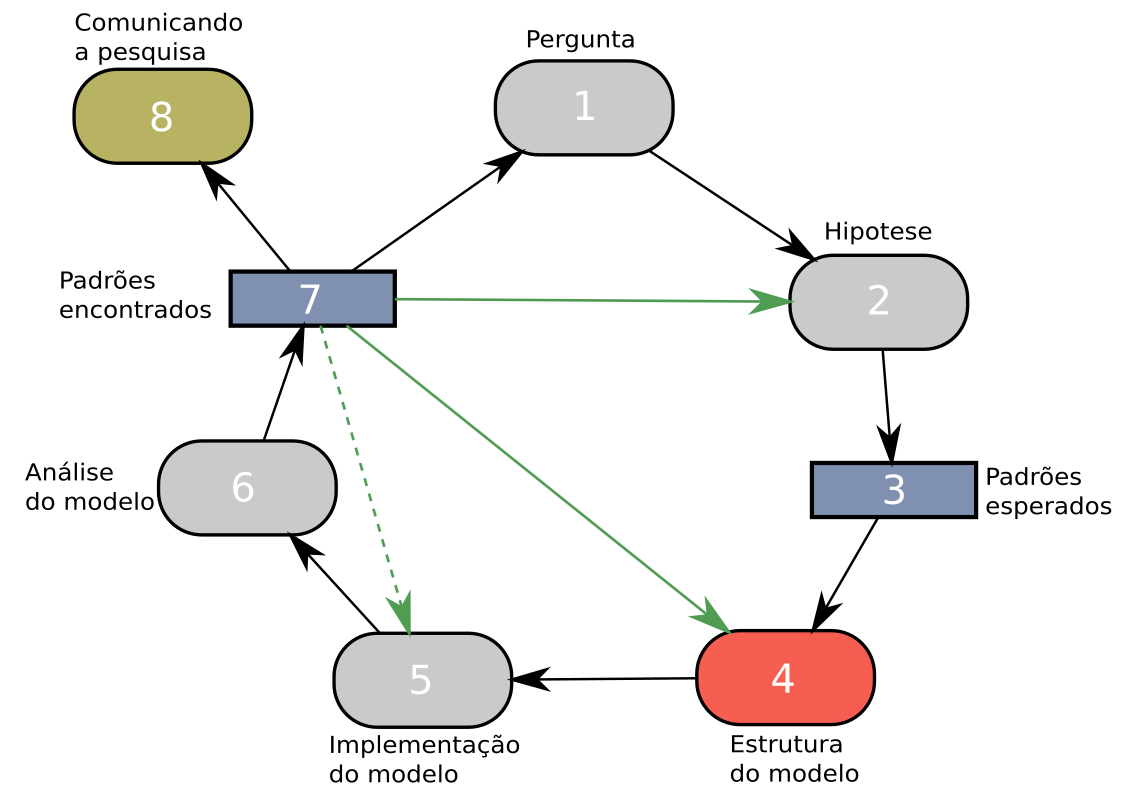
\includegraphics[width=.8\textwidth]{../Figures/intro/Ciclo_Grimm.png}
	\\{\footnotesize Fonte: Elaborada Pelos Autores}
	\label{fig:fluxoGrimm}
\end{figure}

O nó Estrutura do modelo~(4) representa um dos maiores desafios da tese: o de validar uma nova estrutura de modelos. Ao invés de buscar uma ferramenta de modelagem conhecida, pretende-se buscar, dentre as ferramentas conhecidas, aspectos que possam ser aproveitados na formatação de uma estratégia de AM baseada nas ferramentas também conhecidas do \pdcca~e \dmc.

A partir destas suposições, um modelo é implementado~(5) e será trainado e validado de acordo com os critérios de validação de um algoritmo de ML (separação dos dados em treinamento, validação e testes. Montagem da matriz de confusão, etc). O modelo será analisado(6) para verificar se ele repete os padrões esperados de um algoritmo de AM. A linha tracejada que parte do nó 7 para o nó 5 não existe no diagrama de Grimm e Railsback original, mas faz parte da rotina de ajustes de um modelo de AM. Caso se chegue a conclusão que o ajuste não é possível, retorna-se ao nó 4 e se reorganiza as bases utilizadas para criar o modelo. Caso se chegue a conclusão que nenhum ajuste é possível, refaz-se as hipóteses e/ou as perguntas norteadoras. 


\section{Organização da Tese}
\label{sec:organizacao}

A tese será formada pelos seguintes capítulos:
\begin{enumerate}
	\item Introdução
	\item Referencial teórico
	\item Metodologia
	\item Análise dos dados meteorológicos pelo \dmc
	\item Características e validação do modelo de AM proposto
	\item Resultados
	\item Conclusões
\end{enumerate}